\documentclass[12pt,a4paper]{report}
\usepackage[utf8]{inputenc}
\usepackage[french]{babel}
\usepackage[T1]{fontenc}
\usepackage{amsmath}
\usepackage{amsfonts}
\usepackage{amssymb}
\usepackage{graphicx}
\usepackage{xcolor}
\usepackage[pdfauthor={Alexandre MARIN}, pdfkeywords={IFPEN, Delaunay, Voronoi, mesh generation}, colorlinks=true, linkcolor=purple, urlcolor=blue, citecolor=magenta]{hyperref}
%\usepackage{pdfpages}

%\usepackage[nottoc,section]{tocbibind}
\usepackage[defaultbib]{bibtopic}
\renewcommand{\thesection}{\arabic{section}}

\graphicspath{{pictures/}}

\begin{document}

\begin{titlepage}
\author{Alexandre \textsc{Marin}\\ Master Mathématiques et applications Sorbonne Université\\ Parcours Ingénierie Mathématique\\ Majeure Ingénierie Mathématique Pour l'Entreprise}
\date{24/06 -- 30/10/2020\\ Institut Fran\c{c}ais du P\'etrole \'Energies Nouvelles\\ Site de Rueil-Malmaison}
\title{Développement d’une bibliothèque de structures et algorithmes pour un mailleur polyédrique}
\maketitle
\end{titlepage}


\pagenumbering{gobble}
\section*{Remerciements}


\tableofcontents
\newpage

\pagenumbering{arabic}

\section{Introduction}
%1 page
%ouverture
%annonce du plan
%position du stagiaire dans l'entreprise
Ce document est le rapport de mon stage qui a eu lieu à l'Institut Français du Pétrole \'Energies Nouvelles (IFPEN), et clôture donc ma seconde année de master à Sorbonne Université.

Ma position de stagiaire a été la suivante~: j'ai été intégré dans la direction scientifique \emph{Sciences et Technologies du Numérique}, et plus précisément dans le département \emph{Informatique Scientifique} du site de Rueil-Malmaison de IFPEN.

Ce rapport présente d'abord succinctement le déroulement du stage, expose ensuite son contexte en présentant l'entreprise, puis la mission du stage est détaillée et une quatrième partie apporte la conclusion.

Les informations qui concernent l'IFPEN ont été recueillies sur le site internet de l'IFPEN et sur l'intranet de l'entreprise.

\newpage
\section{Déroulement du stage}
%un paragraphe par mois
%une ou deux pages
Le premier mois du stage a été consacré à la découverte des locaux, à certaines formations obligatoires pour les nouveaux salariés (comme la formation sécurité) et à l'installation de logiciels nécessaires pour le stage. \`A la fin du mois de juillet, j'avais pris en main l'environnement de développement intégré QtCreator, une structure de données en demi-arêtes pour des maillages bidimensionnels était programmée en C++ et des maillages de Delaunay pouvaient être générés.

Pendant le deuxième mois, le code C++ a ensuite été réorganisé dans le but d'ajouter plus facilement d'autres fonctionnalités comme le calcul de triangulations de Delaunay contraintes. De nombreux tests ont aussi été effectués pour vérifier la stabilité des programmes ainsi que la qualité des résultats.

Le rapport de stage a été composé lors du troisième mois. Entretemps, des diagrammes de Voronoï étaient générés et le code était amélioré.

\newpage
\section{Contexte et données générales}
%2-3 pages
Cette section a été composée à partir d'informations récupérées sur le site internet de l'IFPEN et sur son réseau intranet.

L'Institut Français du Pétrole -- \'Energies Nouvelles (IFPEN) est une entreprise du groupe du même nom : il s'agit d'un établissement public de recherche et de formation dans les domaines de l'énergie, du transport et de l'environnement, placé sous la tutelle du ministre chargé de l'énergie. IFPEN est financé environ à moitié par l'\'Etat et crée lui-même plus de 50\% de son budget, notamment en valorisant le travail issu de la recherche. L'entreprise est présente sur deux sites : l'un à Rueil-Malmaison en \^Ile-de-France et l'autre à Solaize en Auvergne-Rhône-Alpes.

En 2019, IFPEN comptait $1\ 633$ salariés à temps plein, dont $1\ 136$ ingénieurs et techniciens R\&I (Recherche et Innovation), ainsi que près de $200$ allocataires de recherche, postdoctorants et stagiaires. Son budget atteignait $283,3$~\textrm{M}\texteuro. IFPEN déposait aussi $185$ brevets et est à l'origine de plus de $600$ publications scientifiques et communications à congrès.

IFPEN conçoit et développe des procédés, des équipements et des logiciels qui concernent quatre domaines : la mobilité durable, les énergies renouvelables, les hydrocarbures responsables, et le climat/l'environnement. Dans le domaine climat et environnement, l'une des problématiques est par exemple le captage, le stockage et l'utilisation du CO$_2$. Il s'agit de proposer aux industries lourdes (sidérurgie, cimenterie, raffinage, chimie, pétrochimie) des technologies pour réduire massivement leurs émissions de CO$_2$.

IFPEN collabore avec d'autres instituts de recherche et industries dans le cadre de partenariats qui sont de différents types. IFPEN est ses partenaires financent conjointement un projet de recherche et définissent les règles de propriétés des résultats grâce aux contrats de recherches bilatéraux, aux consortiums dont certains sont des Joint Industry Project (JIP) : IFPEN y opère le programme R\&I et conserve la propriété industrielle. IFPEN participe aussi à des projets de recherche collaborative qui bénéficient de soutiens publics.

La plupart des entités de IFPEN, que l'on peut voir sur la figure \ref{ifpen_org}, se répartissent dans deux ensembles : les directions de recherche, qui rassemblent les compétences scientifiques, et les directions fonctionnelles, comme les ressources humaines, les finances ou le juridique.

Les programmes de recherche sont menés à travers des projets pouvant faire intervenir plusieurs directions de recherche et fonctionnelles. Ces mêmes projets sont pilotés par l'un des cinq centres de résultats qui s'occupent également de leur valorisation industrielle.

On trouve aussi dans l'entreprise une école d'ingénieurs, IFP School, ainsi que la direction générale. Il y a enfin un conseil d'administration, composé de seize membres dont quatre sont des représentants de l'\'Etat venant des ministères de l'énergie, de l'industrie, du budget et de la recherche.

\newpage
\section{Mission du stage}

\subsection{Objectifs}

Ce stage sert de prélude à la thèse \og \emph{Maillage polyédrique de volumes 3D optimisé pour la simulation en géosciences} \fg{}~: l'objectif de cette thèse est de proposer et confronter plusieurs stratégies de génération d'un maillage polyédrique du sous-sol à de nouveaux types de schémas numériques. Afin de rendre possibles des simulations concernant les problématiques du stockage du CO$_2$, la géothermie ou l'hydrogéologie, il faut représenter le plus fidèlement possible les discontinuités et hétérogénéités de la structure des sous-sols qui influencent beaucoup les transferts de masse et d'énergie. Il s'agit donc, étant donnée une description surfacique des éléments en jeu, de mailler un volume en respectant certaines contraintes, comme la conformité ou les rapports de forme des mailles.

Le premier objectif était, d'une part, d'effectuer un travail bibliographique sur la génération de maillages, et d'autre part, de créer une bibliothèque logicielle qui fournisse un maximum d'algorithmes et les structures de données nécessaires au développement du mailleur.

\subsection{Travail effectué}

\subsubsection{\'Eléments théoriques pour les maillages}

Une \emph{triangulation de Delaunay} d'un ensemble de points $V\subset\mathbb{R}^2$ est un maillage conforme de l'enveloppe convexe de $V$, constitué de triangles satisfaisant la propriété du cercle vide~: le disque ouvert défini par le cercle circonscrit d'un triangle ne doit contenir aucun sommet de $V$. Ces triangles sont dits alors Delaunay. Parmi toutes les triangulations de $V$, celles qui sont Delaunay maximisent la valeur du plus petit angle formé par deux arêtes~: ce sont donc, pour cet ensemble $V$ et du point de vue de la qualité des mailles, les \og meilleures \fg{} triangulations.

La propriété de ces maillages s'exprime aussi localement~: un maillage est Delaunay si et seulement si chaque arête est \emph{localement Delaunay}, \emph{i.e.} si chaque arête $e$ est au bord ou bien est la frontière commune de deux triangles $\tau_1$ et $\tau_2$ tels que le cercle circonscrit de $\tau_1$ n'englobe aucun sommet de $\tau_2$.

Lorsque l'on souhaite faire apparaître des arêtes spécifiques d'un ensemble $L$ dans le maillage à obtenir, on peut produire des maillages \emph{Delaunay contraints}~: il suffit pour cela de créer des maillages dont chaque arête est soit dans $L$, soit localement Delaunay. Les éléments de $L$ sont appelés des \emph{segments}.


Le \emph{diagramme de Voronoï} d'un ensemble fini de points $V\subset\mathbb{R}^2$ est constitué d'un ensemble de cellules $V_p$ pour tout $p\in V$, définies par
\[V_p\ :=\ \left\{x\in\mathbb{R}^2\middle\vert\ \forall\,q\in V,\ \Vert x-p\Vert\leqslant\Vert x-q\Vert\right\}\text{.}\]
Il s'agit du dual de la triangulation de Delaunay $\mathcal{T}$ de $V$~: le diagramme de Voronoï relie les centres de cercle circonscrit des triangles de $\mathcal{T}$. Il existe toujours cependant des cellules de Voronoï qui sont infinies et délimitées aussi par des bissectrices des arêtes du bord de $\mathcal{T}$. De façon générale, les cellules $V_p$ sont des polygones convexes.

Lorsque l'on définit en plus l'ensemble des segments $L$ qui doivent apparaître dans le maillage $\mathcal{T}$, on s'intéresse plutôt au diagramme de Voronoï \emph{étendu} $\mathcal{V}$, défini dans \cite[pages 30-31]{Edelsbrunner}. Ici on ne représente que la \og feuille primale \fg{}~: on ne fait pas figurer des arêtes qui relient des centres de cercle circonscrit dans le diagramme $\mathcal{V}$ si elles intersectent un segment de $L$. Les sommets des cellules de Voronoï peuvent alors être des milieux de segments ou des intersections de bissectrices d'arêtes de $\mathcal{T}$ avec d'autres arêtes de $\mathcal{T}$.

Un exemple de diagramme de Voronoï obtenu avec la bibliothèque développée est visible sur la figure \ref{del_vor}.


\subsubsection{Structure de données en demi-arêtes}

Afin de rendre compte de la \emph{topologie} du maillage, la structure de données en demi-arêtes a été mise en \oe{}uvre~: cela consiste à représenter le maillage par un graphe plan orienté. Chaque arête donne naissance à deux demi-arêtes, opposées l'une à l'autre, chacune pointant vers l'une des extrémités de l'arête. Pour se déplacer à l'intérieur de la structure de données, chaque demi-arête $he$ pointe vers une autre demi-arête qui part de la destination de $he$ ; $he$ pointe aussi vers la demi-arête qui lui est opposée. Enfin chaque sommet $v$ pointe vers une demi-arête qui part de $v$ et l'on sait pour chaque demi-arête à quelle face elle appartient.

Ainsi, il est aisé de se déplacer dans le maillage et l'on a accès instantanément à des informations topologiques. Par exemple, on peut facilement parcourir une partie de bord du maillage, connaître les voisins d'un sommet et les arêtes qui lui sont incidentes.

Les algorithmes de génération de maillage ont été écrits en tenant compte des avantages de cette structure.



\subsubsection{Structure de données accélératrice}

Les fonctions programmées étant censées générer de \og grands \fg{} maillages, des nuages de points très denses doivent être constitués~: la  complexité temporelle des algorithmes prend alors toute son importance. Par exemple, pour l'algorithme de Bowyer-Watson, la complexité dépend aussi d'une procédure de localisation de points dans une face du maillage ; dans le cas d'une recherche exhaustive, la complexité de l'étape de localisation est en $O(t)$, avec $t$ le nombre de triangles du maillage. On décide de remplacer cette procédure coûteuse en s'aidant d'un \emph{quadtree}, \emph{i.e.} un arbre quaternaire.

Le principe de la recherche est le suivant~: au préalable, on part d'une boîte $B$ censée englober le maillage et on convient du nombre maximal d'éléments pouvant être contenus dans une feuille de l'arbre. Chaque n\oe{}ud de l'arbre représente une région rectangulaire qui est une portion de la boîte englobante $B$. Lorsque qu'une feuille contient trop d'éléments, on lui crée quatre fils qui correspondent chacun à un quart de la zone représentée par l'ancienne feuille, puis on répartit les éléments dans les nouvelles feuilles selon leur position dans la région. Ainsi, la complexité de la recherche d'un élément selon sa position est en $O(h_{\text{quadtree}})$, avec $h_{\text{quadtree}}$ la hauteur de l'arbre construit.

\subsubsection{Algorithmique}
Dans la bibliothèque à concevoir, on a ajouté des algorithmes de natures différentes qui construisent des maillages de Delaunay, contraints ou non. On y trouve l'algorithme de Bowyer-Watson qui transforme un maillage Delaunay en une autre triangulation de Delaunay en insérant un nouveau sommet, par retriangulation locale. On peut aussi décrire un polyèdre général à trous et définir des arêtes et points intérieurs à ce polyèdre, et ensuite obtenir un maillage Delaunay contraint qui tient compte de toutes ces données grâce à l'algorithme d'emballage cadeau, dit \emph{Gift-Wrapping}~: pour cela on part des arêtes du bord et on ajoute au fur et à mesure des triangles Delaunay en avançant vers l'intérieur du domaine à mailler. Il s'agit d'une méthode de génération de maillage faisant partie de la classe d'\emph{avance de front}.

Des variantes de ces algorithmes ont été mises en \oe{}uvre. Pour ajouter un nouveau segment dans un maillage Delaunay contraint, il suffit de supprimer les triangles intersectés par ce nouveau segment et de retrianguler la cavité ainsi formée de part et d'autre du segment ajouté.
Pour insérer un nouveau sommet à l'extérieur d'un maillage que l'on veut garder Delaunay, il suffit d'ajouter quelques triangles au bord et d'invoquer l'algorithme de Bowyer-Watson à partir d'un triangle intérieur.

\subsubsection{Bibliographie et mise en \oe{}uvre informatique}

La bibliographie servant de point de départ se trouve à la fin du rapport, en page \pageref{biblio}. L'article \cite{Garimella} décrit une procédure qui génère des maillages de volumes séparés par des interfaces, à partir des diagrammes de Voronoï. Puisqu'il faut au préalable déterminer des triangulations de Delaunay, les notes \cite{delnotes} ont été lues pour avoir à disposition des algorithmes de génération de maillages de Delaunay. Le livre \cite{Edelsbrunner} complète les deux premières références, en donnant par exemple la définition des diagrammes de Voronoï étendus pour les maillages de Delaunay contraints.

La bibliothèque logicielle à créer a été programmée en C++ à l'aide de l'environnement de développement intégré QtCreator \cite{QtCreator}. Cette bibliothèque est découpée en plusieurs sous-projets que l'on présente ici~:
\begin{description}
\item[noyau géométrique]~: cela permet d'effectuer des calculs en géométrie. La bibliothèque Eigen \cite{Eigen} écrite en C++ a été incorporée au projet pour faire de l'algèbre linéaire ;
\item[maillages bidimensionnels]~: on utilise la structure en demi-arêtes pour représenter les maillages dans le plan ;
\item[entrées/sorties]~: afin de visualiser ou réutiliser des maillages, l'importation et/ou l'exportation a été codée pour les formats \verb+OBJ+ et \verb+PLY+ ;
\item[Delaunay]~: ce projet fournit des algorithmes pour générer des triangulations de Delaunay et de Delaunay contraintes ;
\item[Voronoï]~: ce projet permet de calculer des diagrammes de Voronoï ;
\item[tests]~: dans ce dernier sous-projet, on y prépare des cas tests pour valider les programmes et pour s'assurer que ces derniers sont stables, rapides et/ou suffisamment précis.
\end{description}

La gestion de version s'est faite grâce à l'outil Git \cite{Git}.

\subsection{Résultats}


\subsection{Problèmes rencontrés}

%visualisation-couleurs
%bogues
La principale difficulté a été la vérification des fonctions programmées par la visualisation des résultats obtenus. Différents logiciels ont été utilisés, comme Paraview, CloudCompare ou MeshLab \cite{Paraview, CloudCompare, MeshLab}, mais ils n'interprètent pas tous les mêmes formats de fichier et ils peuvent rendre compte des maillages très différemment. Par exemple, le format \verb+PLY+ permet de renseigner des couleurs attachées à des points, arêtes et faces ; cependant ces données ne sont pas toujours acceptées et souvent les éléments sont coloriés par interpolation des couleurs des extrémités, ce qui ne correspond pas tout le temps à ce que l'on veut obtenir. Néanmoins ces couleurs se sont révélées pratiques quand il a fallu afficher des propriétés comme celle d'être localement Delaunay pour une arête.

\newpage
\section{Conclusion}

\newpage
\section{Annexes}

\begin{center}
\begin{figure}[htbp]
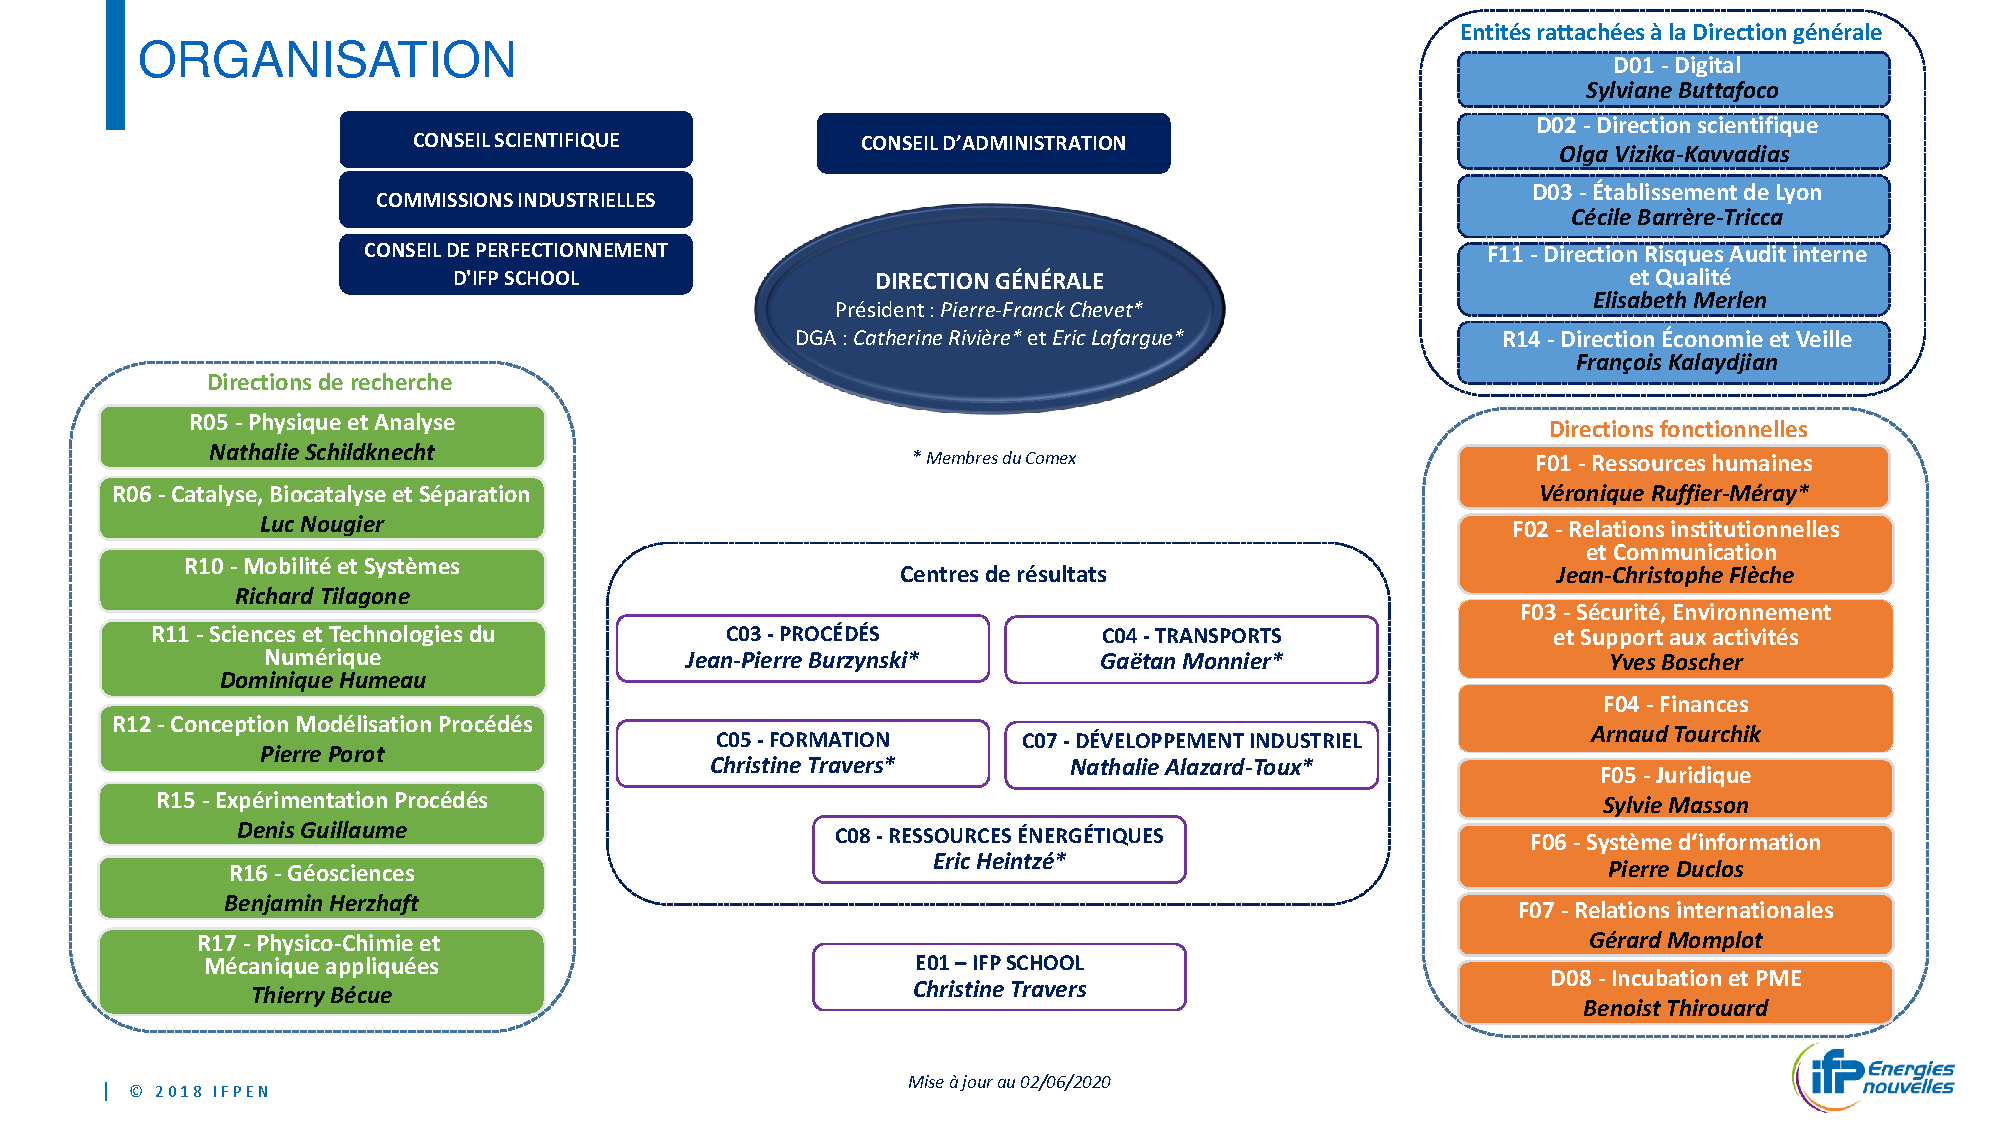
\includegraphics[scale=0.6, angle=90]{vf-schema-organisation-ifpen-marguerite.pdf}
\caption{Schéma de l'organisation de l'IFPEN (source : intranet de l'IFPEN)}
\label{ifpen_org}
\end{figure}
\end{center}
\clearpage

\begin{center}
\begin{figure}[htbp]
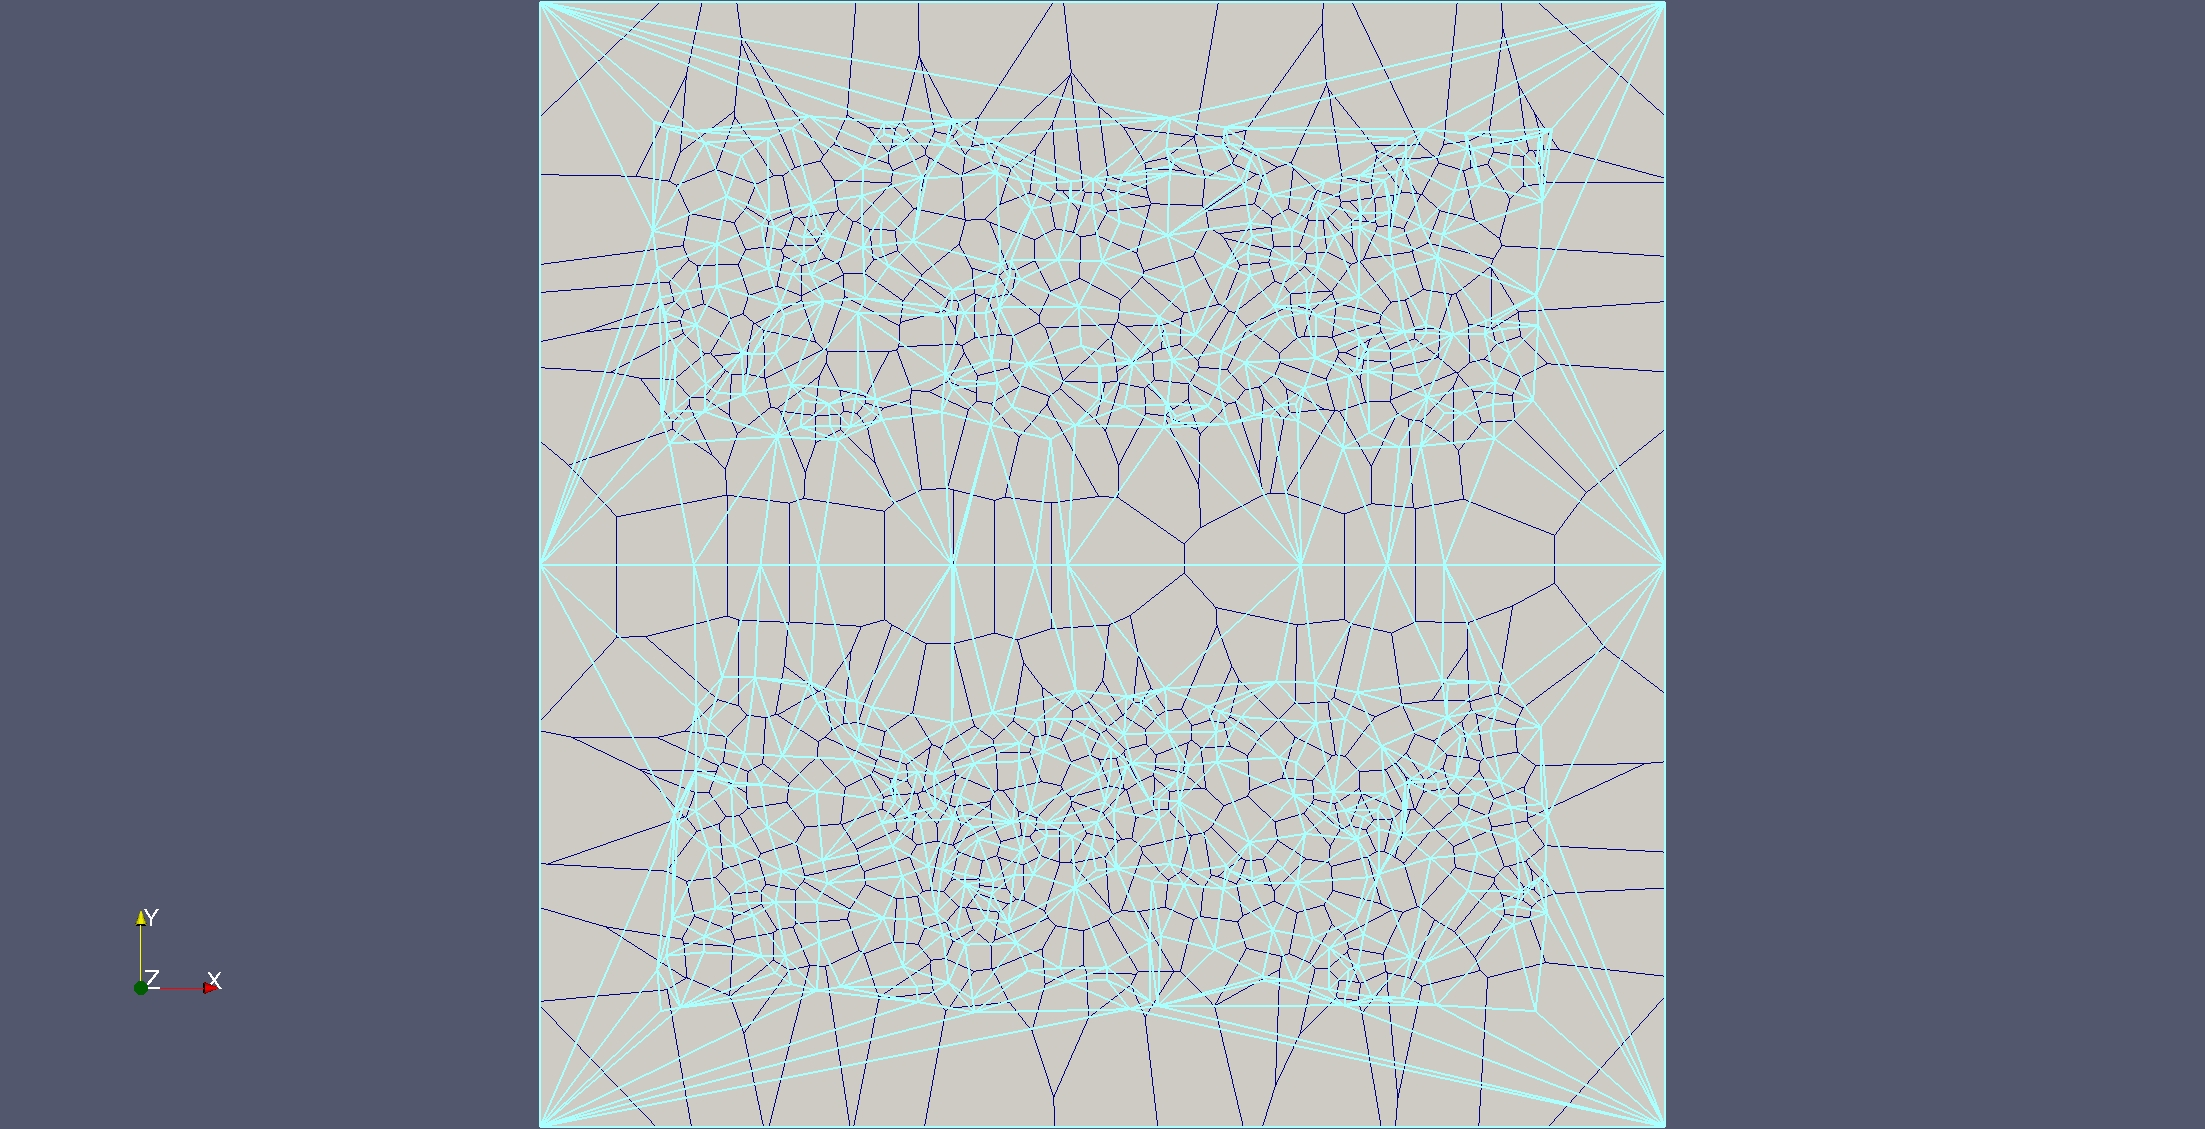
\includegraphics[scale=0.35, viewport=530 0 1680 1129, clip]{del_vor.jpg}
\caption{Triangulation de Delaunay (arêtes en bleu clair) et diagramme de Voronoï correspondant (arêtes en bleu foncé) (image obtenue avec Paraview)}
\label{del_vor}
\end{figure}
\end{center}
\clearpage


\section{Références}
\vspace*{1cm}

\bibliographystyle{plain}
\begin{btSect}{doc}
\section*{Bibliographie}
\btPrintCited
\end{btSect}
\label{biblio}

\bibliographystyle{plain}
\begin{btSect}{software}
\section*{Logiciels}
\btPrintCited
\end{btSect}
\label{software}

\end{document}
